\chapter{
Modeling Space Usage:
Integrating Resource Selection Information with
Spatial Capture-Recapture
  Models}

\markboth{Chapter XXX}{}
\label{chapt.rsf}


\vspace{.3in}

Up to this point we have developed many specific variations of
relatively simple SCR models. They included different models of the
observation process, models of the relationship between encounter
probability and distance, and different types of covariates including
behvioral responses and other things that should affect detection
probability.  That said, the models remain pretty basic in the sense
that they imply simplistic models of how individuals use space
(section \ref{scr0.sec.implied}) and how individuals are distributed
in space.  In the following several chapters we generalize some of the
core SCR assumptions to accommodate more realistic notions of how
animals use space.

In this chapter we extend our notion of encounter probability models
as models of resource selection (sec. \ref{scr0.sec.implied}), by
extending them to included explicit landscape covariates. We do this
in a way that is entirely consistent with the manner in which
classical ``resource selection function'' (RSF) models are estimated
from animal telemetry data.  In fact, we argue there that SCR models
and ``RSF/telemetry'' models have the same basic underlying model of
space usage, just that in the SCR model encounter of individuals is
imperfect (i.e., $p<1$) whereas RSF data obtained by telemetry is
perfect (i.e., p=1). We can think of the two as being exactly
equivalent either if we have a dense array of trapping devices, or if
our telemetry apparatus is imperfect (fails a large percentage of the
time, randomly).  A key conceptual thing is we need to formulate both
the SCR model and the RSF model in terms of a common latent variable
so that we can make them consistent with respect to some underlying
space utilization process.


Here we show how to integrate standard RSF type data into SCR models
to model space usage explicitly. This produces asymmetric, irregular
and non-stationary home ranges, and allows us to make formal
inferences about factors that influence home range geometry and
morphology directly from SCR data.  We begin by describing a model for
space usage that exists independent of how we obtain the data. Then we
introduce observation models consistent with both standard
capture-recapture methods and telemetry.  This allows us to define a
general likelihood function that is the product of the two
components, if they are both simultaneously available.  In the absence
of RSF data from telemetry, the model reduces to an ordinary SCR model
but with a spatial covariate
\hl{ Can you clarify? What kind of spatial covariate? Is it necessary?
I'm sure it is explained shortly, but at this point it isn't entirely clear.}
on encounter probability.  In summary,
the framework allows us to estimate RSFs directly from SCR data, or to
integrate telemetry data directly into SCR models.

XXXX below par goes elsewhgere XXXXX

In our formulation we estimate the latent ${\bf s}$ variables from the observed telemetry
data, just as a convenience, but this wouldn't be necessary.
Also we assume the data are independent pieces but if some of the SCR
individuals are the same as the telemetered individuals then we should
probably account for that explicitly. So right now we pretend we don't
know anything about the telemtered guys in terms of their capture
history. So they don't contribute to information about baseline
encounter probability, just to estimates of the other encounter model
parameters.



\section{Basic Model of Space Usage}
\label{rsf.sec.rsfmodel}

We develop the model here in terms of a discrete landscape purely for
computational expediency. That said, essentially no landscape on your
computer is continuous, the one exception is if the landscape is
defined strictly in terms of variables that themselves are inherently
continuous -- e.g., ``distance to road'' or something like that.  But
almost all habitat or landscape structure data comes to us in the form
of raster data.  Let $x_{1},\ldots,x_{nG}$ identify the center
coordinates of a set of $nG$ pixels that define a landscape. ({\bf
  consistent with other notation?}) We organize them into a matrix
${\bf X}_{nG \times 2}$.  Let $z(x)$ denote a covariate defined for
every pixel $x$.

We suppose that a population of individuals wanders around space in
some manner related to the covariate $z(x)$, and their locations
accumulate in pixels by some omnipotent accounting mechanism. Let
$n_{ij}$ be the number of times individual $i$ used pixel $j$ during
some period of time.  We assume the following probability mass
function for the distribution of ``use'' -- the number of occurrences
of individual $i$ in pixel $j$:
\[
{\bf n}_{i} \sim \mbox{Multinom}({\bm \pi}_{i})
\]
where
\[
 \pi_{ij} = \frac{ exp( -\alpha_{2} z(x) ) }{ \sum_{x} exp(-\alpha_{2} z(x))}
\]
This is the standard RSF model \citep{manly_etal:2002} used to model
telemetry data.  In practice, we don't get to observe $n_{ij}$ for all
individuals but, instead, only for a small subset which we capture and
install telemetry devices on.  For these telemetered individuals we
accumulate individual- and pixel-specific frequencies, at a lower
sampling rate than actual individual use. For example, we might choose
to record the location of an individual every hour or day or
whatever. As such, the observed frequency of pixel use is a sample
but, if the recording is random or systematic (or otherwise unrelated
to {\it where} individuals are located), then we can imagine that the
same model of space usage applies. (formally, we suppose that the
observed frequencies are a binomial sample with sample size $n_{ij}$
and sampling intensity $\alpha_{0}$ lets say, and we see that the
constant $\alpha_{0}$ cancels from the expression for the multinomoial
cell probabilities above).

For the telemtered individuals then,
we adopt the standard RSF
model which has probabilities as above:
\[
 \pi_{i,j} = \frac{ exp( -\alpha_{2} z(x) ) }{ \sum_{x} exp(-\alpha_{2} z(x))}
\]
We could have multiple such covariates but we focus on a
single covariate here for clarity.  We extend this model slightly to
make it more realistic spatially. Let ${\bf s}$ denote the centroid of
an individuals home range and let $D_{ij}$ be the distance from ${\bf
  s}_{i}$ to pixel ${\bf x}_{j}$. We modify the space usage model to
accomodate that space use will be concentrated
around an individuals home range centroid:
\[
 \pi_{i,j} = \frac{ exp( -\alpha_{1} D_{ij}^{2} -\alpha_{2} z(x) ) }
{ \sum_{x} exp(-\alpha_{1} D_{ij}^{2} -\alpha_{2} z(x))}
\]
In this case, if you have no covariates at all, or if $\alpha_{2} =
0$, then
the probabilities $\pi_{ij}$ are directly proportional to the SCR
model for encounter probability.
For example, setting $\alpha_{2} = 0$, then this implies probability
of use for pixel $j$ is:
\[
p_{ij} \propto  exp( -\alpha_{1} D_{ij}^{2})
\]
so whatever function of distance we use in our RSF implies an
equivalent model of space usage when used in SCR models.

As an illustration of space usage patterns under this model, we
simulated a covariate that we feel represents typical habitat
structure (Fig. \ref{rsf.fig.habitat}). This was simulated by using a
basic kriging model with the following commands:
\begin{verbatim}
set.seed(1234)
gr<-make.grid(minx=1,maxx=40,miny=1,maxy=40,nx=40,ny=40)
Dmat<-as.matrix(dist(gr))
V<-exp(-Dmat/5)
z<-t(chol(V))%*%rnorm(1600)
spatial.plot(gr,z)
\end{verbatim}
The functions \mbox{\tt make.grid} and \mbox{\tt spatial.plot} are
both in the \mbox{\tt scrbook} package \hl{I think people would prefer
  to work with existing/familiar plot functions, like the ones in the raster
  package or in the sp package}.  We show an example of space
usage for 8 individuals ....... in Fig. \ref{rsf.fig.homeranges},
simulated with $\alpha_{1} = 1/(2\sigma^2)$ with $\sigma = 2$ and the
coefficient on $z(x)$ set to $\alpha_{2} = 1$.  These exhibit clear
non-stationarity in response to the structure of the underlying
covariate and are distinctly asymmetrical.  We note that if
$\alpha_{2}$ were set to 0, the 8 home ranges shown here would equate
precisely to bivariate normal kernels with $\sigma = 2$.  Another
interesting thing to note is that the activity centers are not
typically located in the pixel of highest use or even the centroid of
usage.

\begin{figure}[htp]
\centering
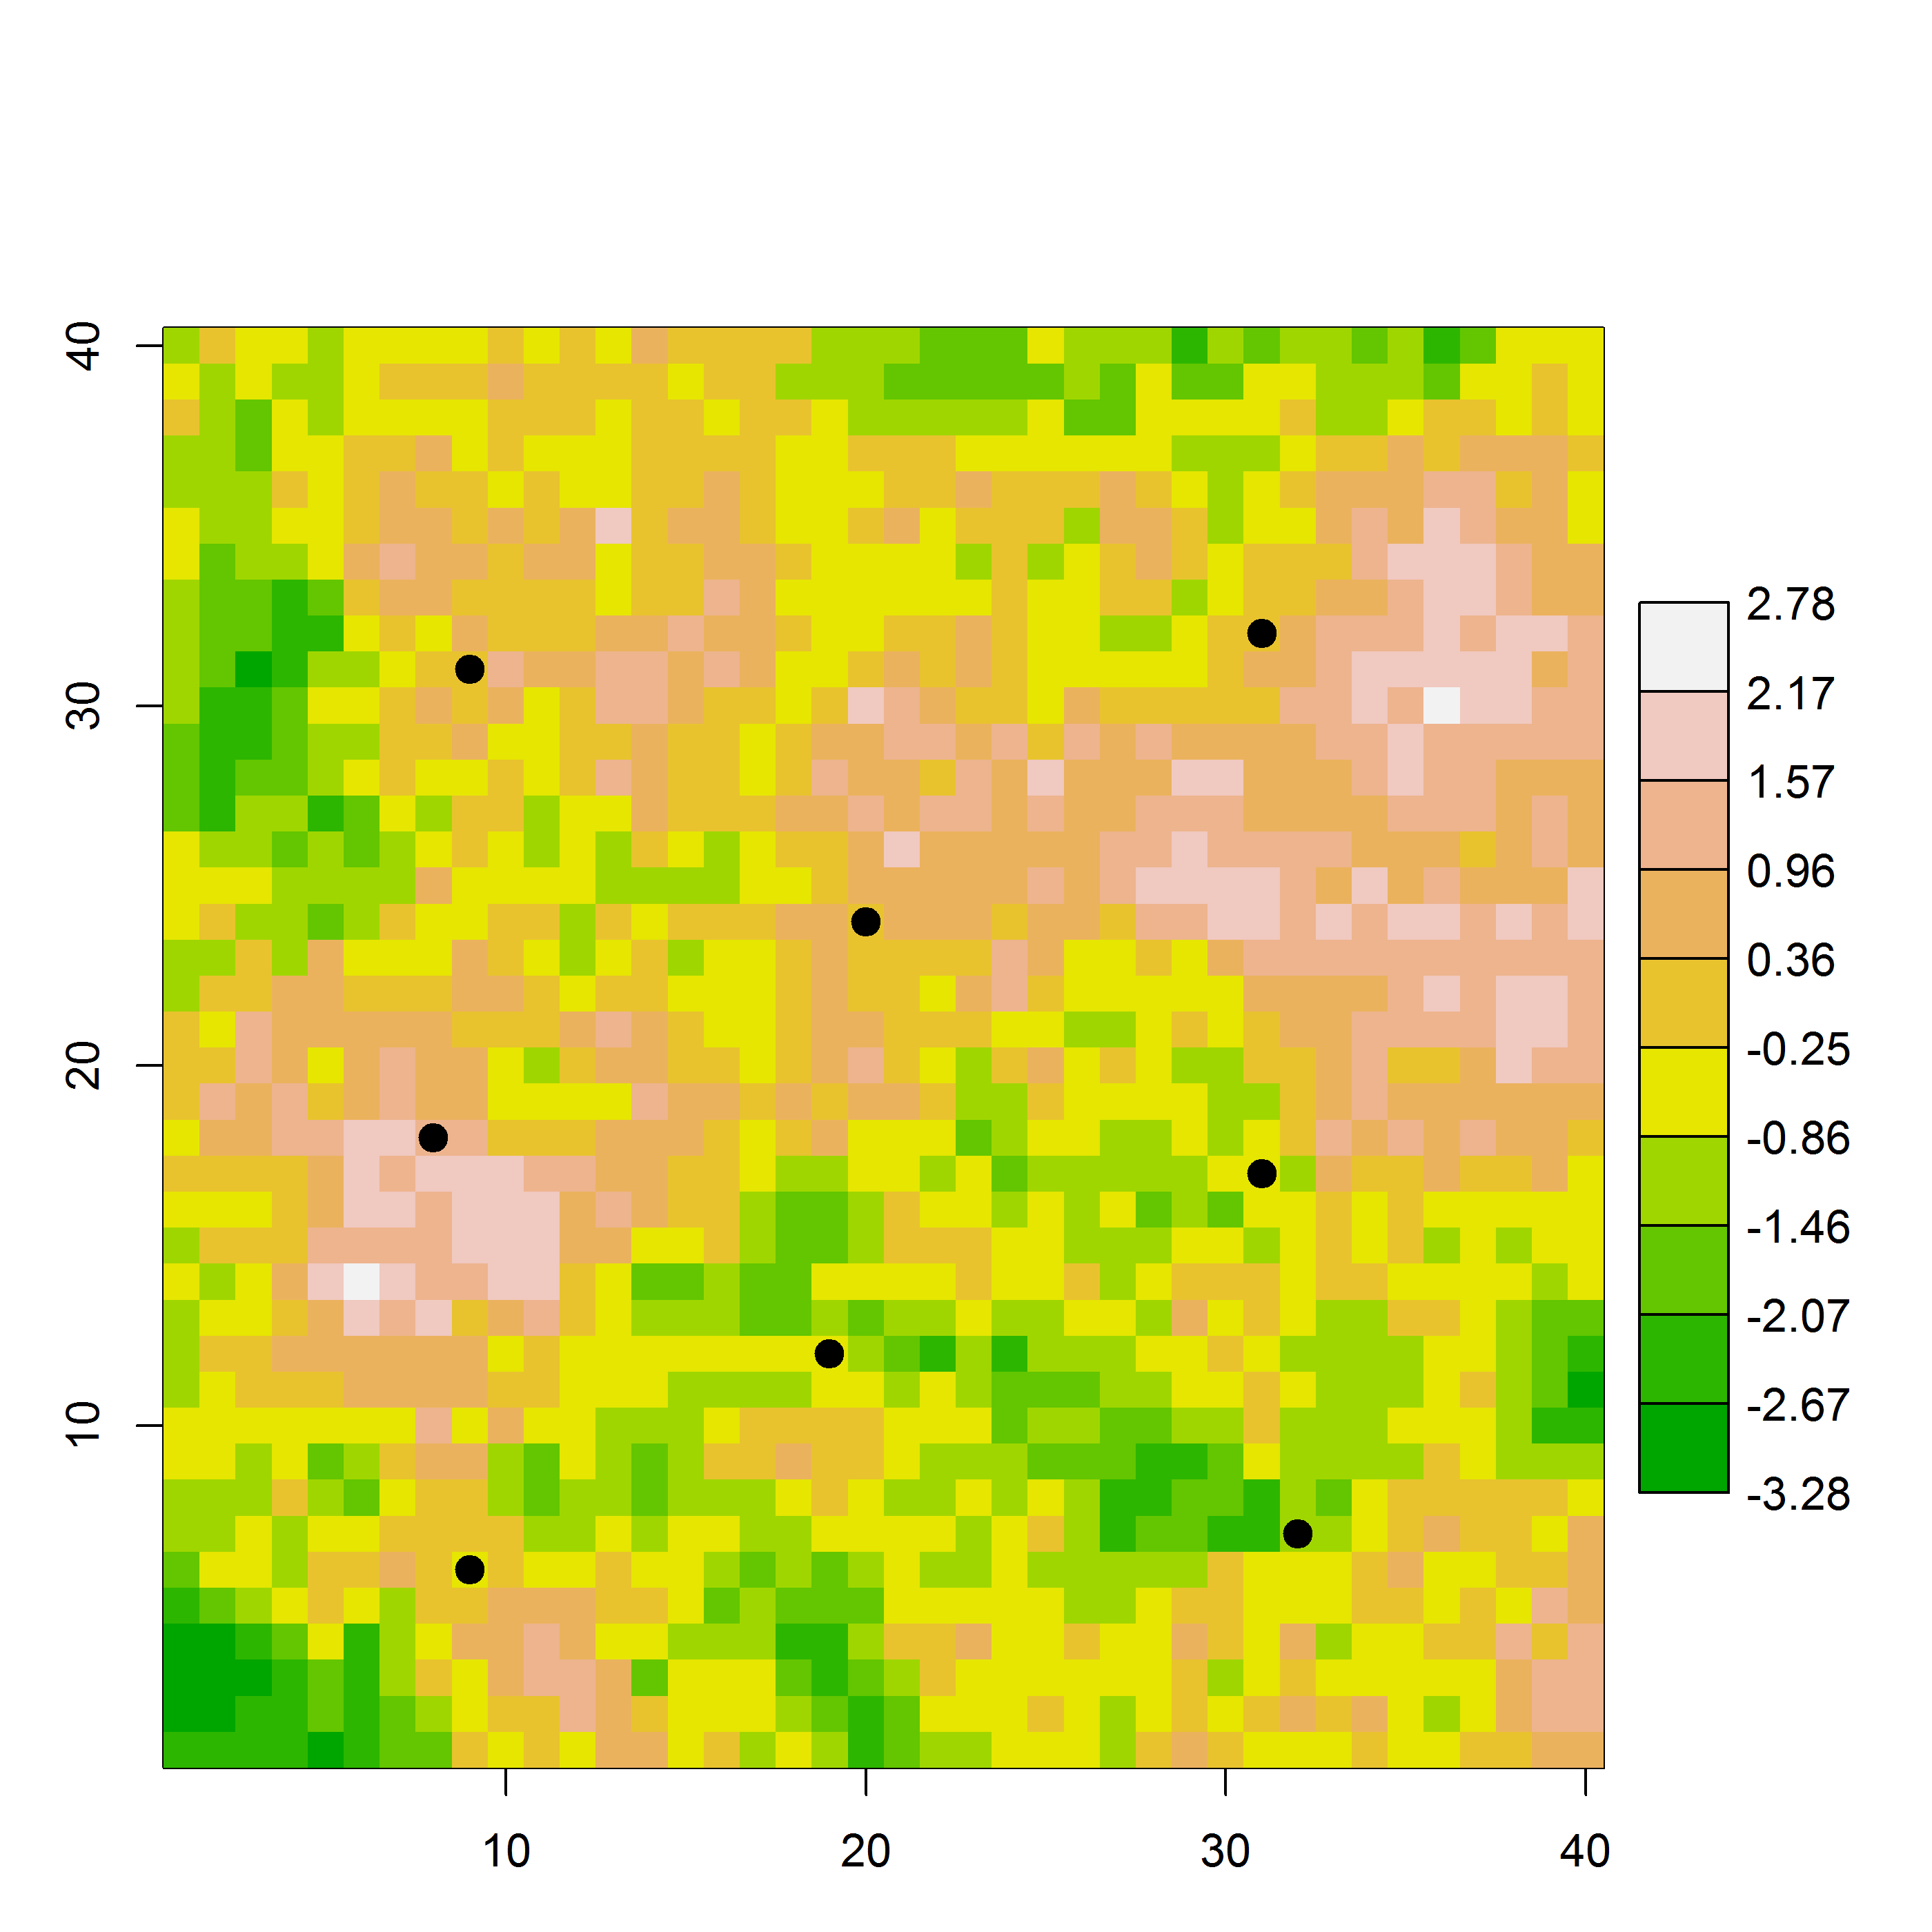
\includegraphics[width=4in,height=4in]{Ch10b/figs/habitat}
\caption{A habitat covariate. Home range centers for 8 individuals are
shown with black dots.}
\label{rsf.fig.habitat}
\end{figure}


\begin{figure}[htp]
\centering
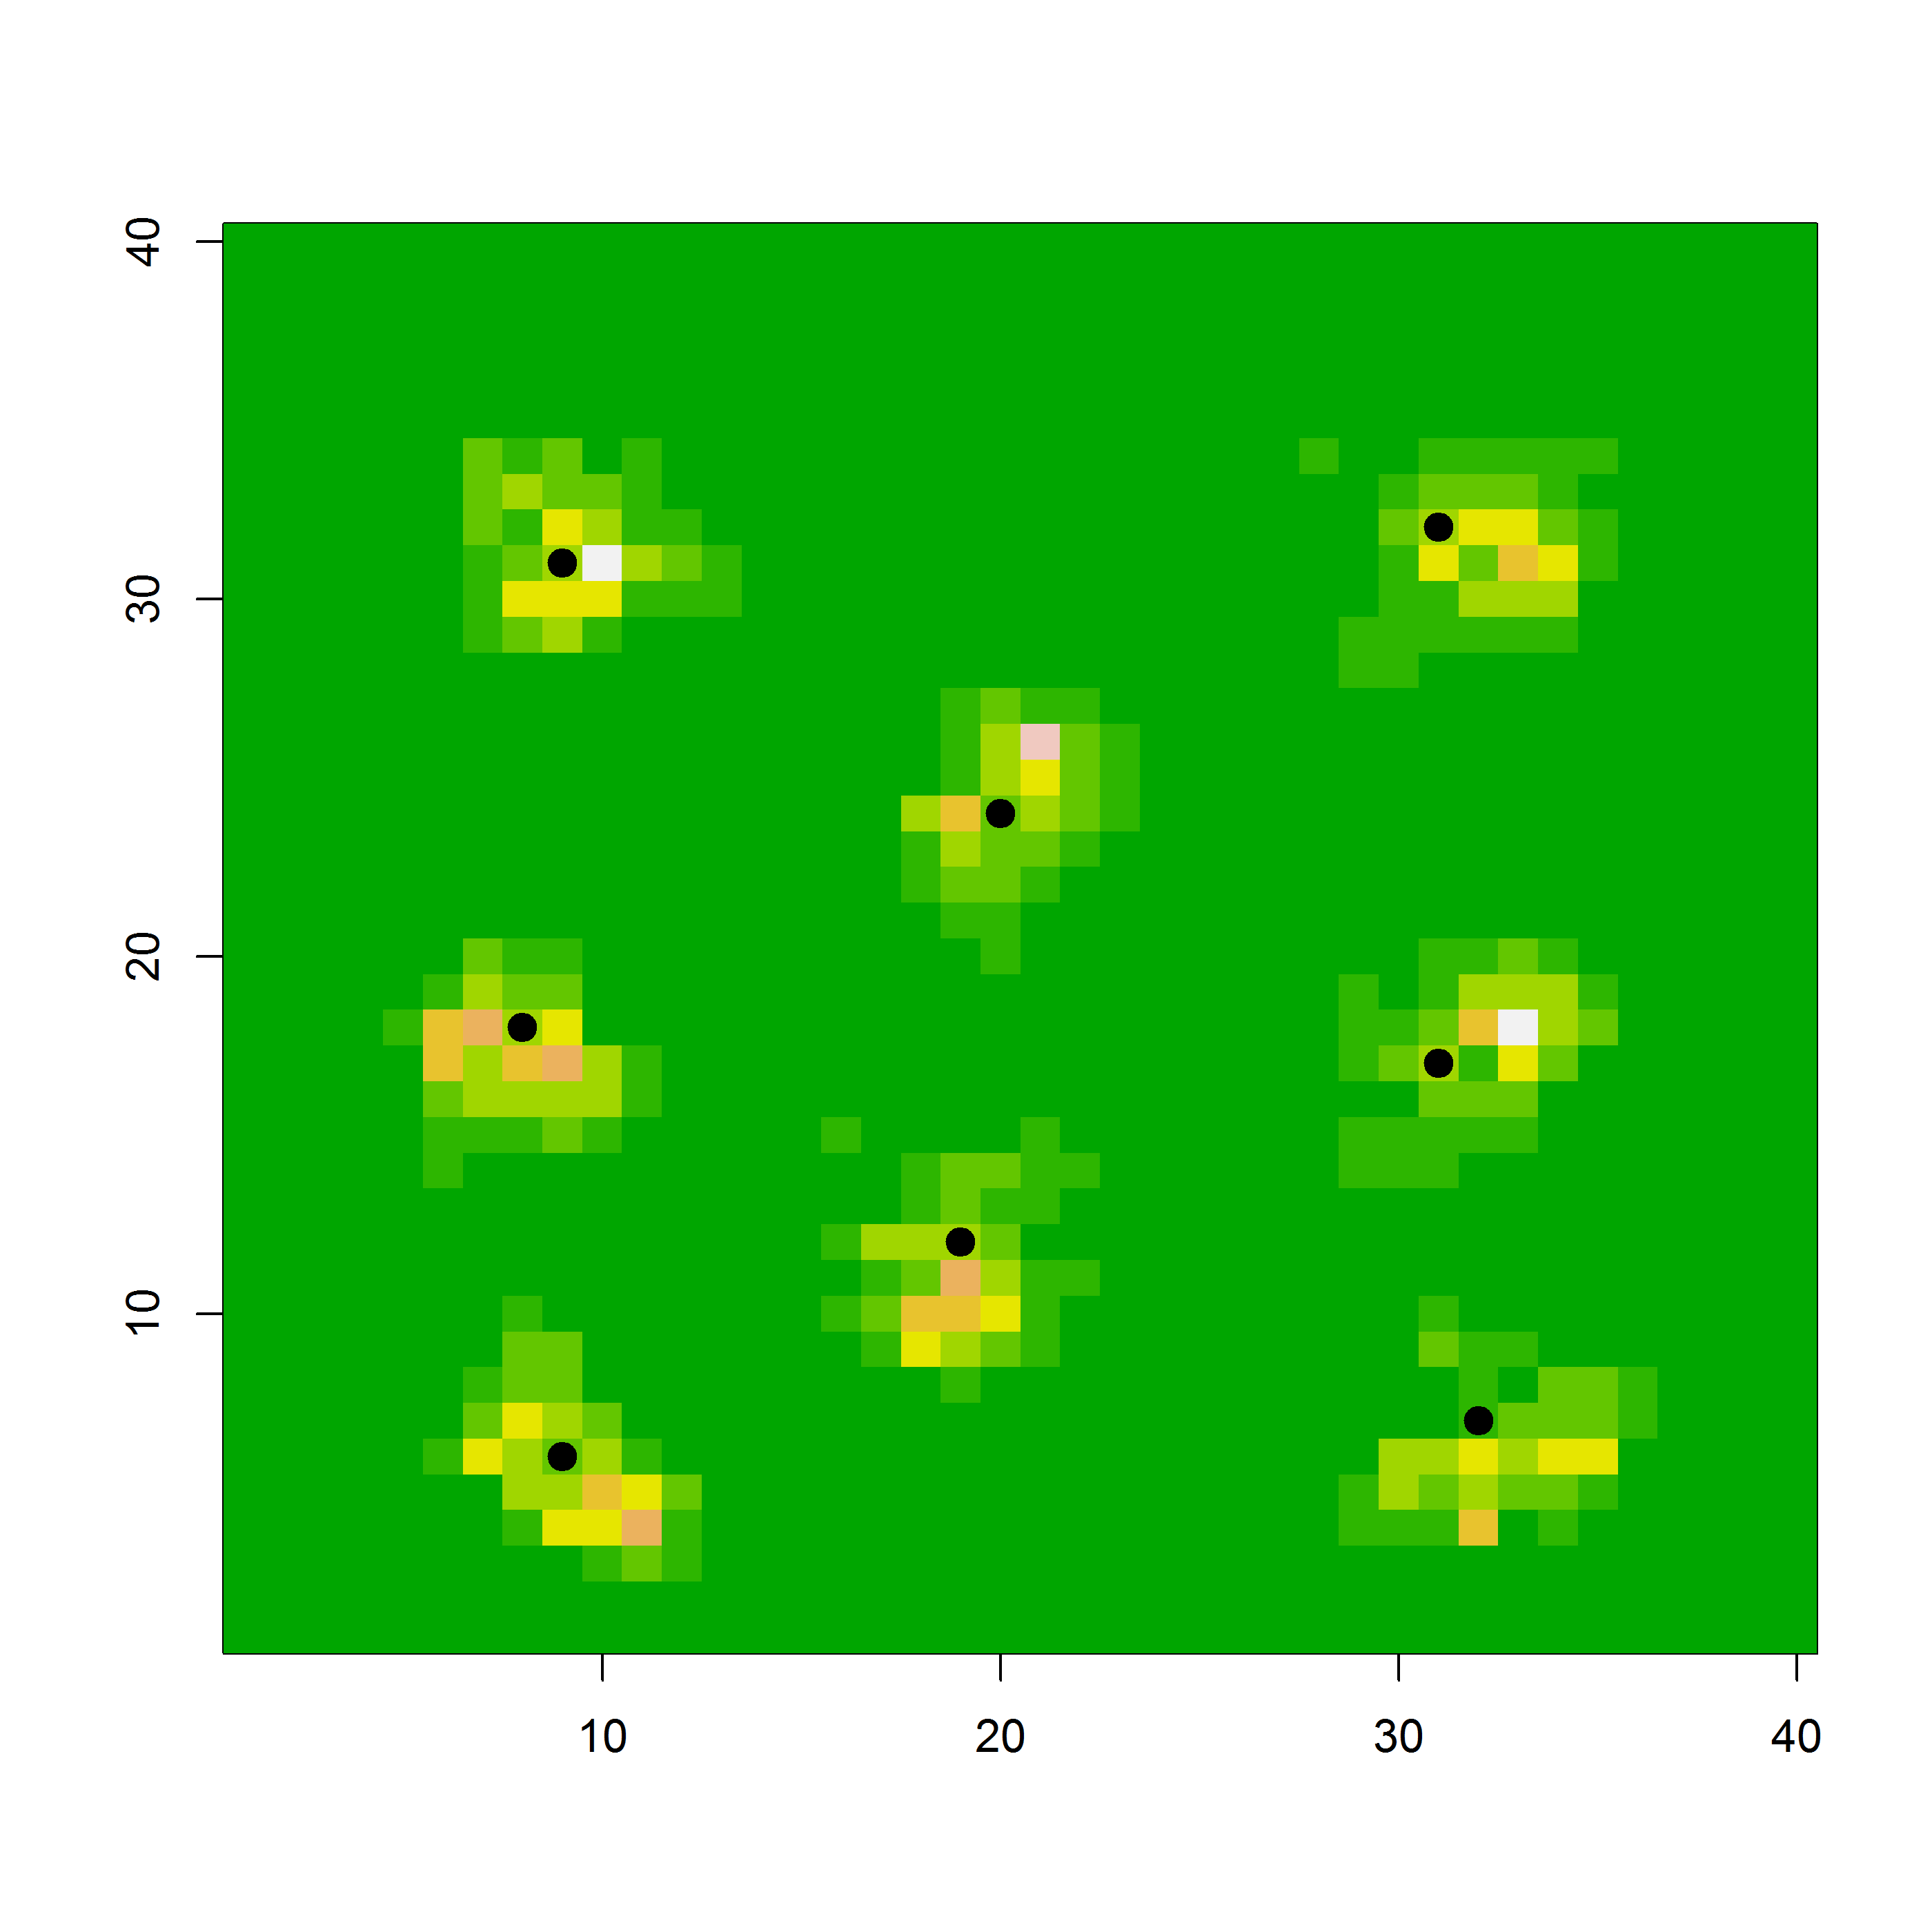
\includegraphics[width=4in,height=4in]{Ch10b/figs/homeranges8}
\caption{Space usage patterns of 8 individuals under a space usage
  model that contains a single covariate (shown in
  Fig. \ref{rsf.fig.habitat}).
}
\label{rsf.fig.homeranges}
\end{figure}



\subsection{Poisson use model}

A natural way to movitate this specific model is to
assume that individuals make a sequence of random resource selection
decisions so that the outcome of $n_{ij}$ are marginally {\it
  independent}, having a Poisson distribution:
\[
 n_{ij} \sim \mbox{Poisson}( \lambda_{ij})
\]
where
\[
 log(\lambda_{ij}) = a_{0}  + \alpha_{2} z(x)
\]
In this case,
 the number of visits to any particular cell is affected by
the covariate $z(x)$ but has a baseline rate ($exp(a_{0})$) related to the amount
of movement, or number of selection decisions which is essentially
just related to the time interval over which the animal is using
space. i.e., longer time intervals lead to higher values of
$E(n_{ij})$.
This is an equivalent model to the multinomial model given previously
in the sense that, if we condition on the total sample size $n_{i.} =
\sum_{j} n_{ij}$, then the vector ${\bf n}_{i}$ has a multinomial
distribution with probabilities
\[
 \pi_{ij} = \frac{\lambda_{ij}}{ \sum_{j} \lambda_{ij}}
\]
as we discussed in Chapt. \ref{chapt.poisson-mn}.  We see that the
intensity parameter $a_{0}$ is not relevant for understanding
patterns of space usage.

For purposes of estimation we can use either the Poisson or
multinomial likelihoods. In the former case, we estimate the nuisance
parameter $a_{0}$, from which information is derived by the total
number of observations whereas, in the later case, we lose information
about $a_{0}$ by conditioning on the total (i.e., treating it as
fixed).  As it often is fixed, or at least the number of telemetry
observations is completely arbitrary, $a_{0}$ is usually a meaningless
parameter so whether we estimate it or not is immaterial from a
practical standpoint.


\subsection{Thinning}

Suppose our sampling is imperfect so that we only observe a smaller
number of fixes than $n_{ij}$. As in sec. \ref{scr0.sec.implied}, we assume
\[
 m_{ij} \sim \mbox{Bin}(n_{ij}, \phi_{0}).
\]
In this case, the marginal distribution of $m_{ij}$ is also Poisson
but with intensity $\lambda_{0} = log(\phi_{0}) + a_{0} +
\alpha_{2}z(x)$.  In this case, the space-usage model (RSF) for the
thinned counts $m_{ij}$ is the same as the space-usage model for the
original variables $n_{ij}$.  This is because if we remove $n_{ij}$
from this model by summing over possible values, then the vector of
${\bf m}_{i}$ has a multinomial with cell probabilities
$\lambda_{0}\pi_{ij}$ and we see that $\lambda_{0}$ cancels.

%That is,
%given our sequence of
%independent Poisson random variables and we condition on their total,
%i.e., regard it as fixed, then we have the multinomial. In the
%multinomial we lose information about the intercept which in this case
%is ok because we only care about the interpretation of the resource
%selection model as a probability distribution and don't care about the
%basic rate of detection -- and it is a confounding of animal use and a
%fixed sampling intensity.

In summary, if we conduct a telemetry study we observe ${\bf n}_{i}$,
the $nG \times 1$ vector of pixel-counts for each individual
$i=1,\ldots,N_{tel}$.  We declare these data to be
``resource-selection data'' which are typical of the type used to
estimate resource-selection functions (RSFs) XXX REF XXXXX. Sometimes
in RSF modeling activities people make believe they have continuous
covariates and so the denominator in XXXX involves some kind of
integration over a distribution for the covariate. However, in a
discrete landscape, entertaining pdfs for the covariates isn't
necessary \citep{royle_etal:2012mee}.\hl{Or is it that they ignore the
  fact that they are sampling 2D space? They seem to act as if they
  are sampling K-dimensional covariate space.}


\subsection{SCR Data}

The key to combing RSF data with SCR data is to work with this
underlying resource utilization process and formulate SCR models in
terms of that process. For SCR models it will serve as a intermediate
latent that we don't get to observe. We assume that, fundamentally,
both telemetered individuals and SCR individuals are using space
according to the same resourc selection model. The difference is that,
for SCR data, we dissolve out most of the sampling devices so that
data are only recorded at a subsample of them.
In other words, imagine that we have a sampling device, such as a
camera trap, in {\it every} pixel. If the device operates continually
then it is no different from a telemetry instrument. If it
operates  intermittently and does not expose the entire area of
each pixel then a reasonable model for this imperfect observation is
the ``thinned'' binomial model given above, where $\lambda_{0}$
represents the sampling effectiveness of the device. So we imagine
that the hypothetical perfect data from a camera trapping study are
the counts $m_{ij}$.

We then construct our SCR encounter probability model based on the
view that these frequencies $m_{ij}$ are {\it latent}. In particular,
under the SCR model with binary observations,
 we observe a random variable
$y_{ij} = 1$  if the individual $i$ visited the pixel
containing a trap and was detected.
We imagine that $y_{ij}$ is related to the latent variable $m_{ij}$ being the
event $m_{ij}>0$, which occurs with probability
\[
 p_{ij} = 1-exp(- \lambda_{0} \lambda_{ij})
\]
we see that $\lambda_{0}$ is a baseline encounter rate which includes
the constant intensity of use by the individual and also the baseline
rate of detection conditional on use.



\section{The likelihood}

To construct the likelihood for SCR data when we have auxilliary
covariates on space usage {\it or} direct information on space usage
from telemetry data, we regard the two samples (SCR and RSF) as
independent of one another. In practice, this might not always be the
case but (1) often time the telemetry data come from a previous study;
(2) the individuals are not the same at all; (3) or even if they are
some of the same individuals being captured, we might not be able to
match individuals captured by a sampling method such as hair-snares
with the individuals wearing radio-collars; (4) In cases where we {\it
  can} match individuals between the two samples, regarding them as
independent should only entail an incremental loss of efficiency
because we are disregarding more precise information on a small number
of activity centers.
Anyhow, regaridng the two data sets independently, our approach here
is to form the likelihood for each set of observations as a function
of the same underlying parameters and then combine them. In
particular, let ${\cal L}_{scr}(\alpha_{0}, \alpha_{1}, \alpha_{2}, N;
{\bf y}_{scr})$
be the likelihood for the SCR data in terms of the basic encounter
probability parameters and the total (unknown) population size $N$,
and let ${\cal L}_{rsf}(\alpha_{1},\alpha_{2}; {\bf m}_{rsf})$ be the
likelihood for the RSF data based on telemetry which, because the
sample size of such individuals is fixed, does not depend on $N$. We
might use the Poisson formulation of this likelihood as discussed in
sec. XXXX in which case
we also formally estimate the nuisance parameter $a_{0}$ instead of
conditioning on the total.
The
joint likelihood is the product of these two pieces:
\[
{\cal L}(\alpha_{0},\alpha_{1},\alpha_{2},N; {\bf y}_{scr},{\bf
  m}_{rsf})  = {\cal L}_{scr} \times {\cal L}_{rsf}
\]
In what follows, we provide a formulation of each likelihood
component, along with an {\bf R} function for obtaining the MLEs of
model parameters using standard methods available in {\bf R}.

The observation model for the SCR data based on
sampling over $K$ periods  is:
\[
 y_{ij}|{\bf s}_{i} \sim \mbox{Bin}(K; p_{ij})
\]
where
\[
 p_{ij} = 1-exp(- \lambda_{ij} )
\]
and
\[
 \lambda_{ij} = \lambda_{0} exp(- \alpha_{1} D_{ij}^{2} + \alpha_{2}  z(x_{j}) )
\]
 A compact expression of these
model components is:
\begin{equation}
y_{ij}| {\bf s}_{i} \sim \mbox{Bin}(K, p_{\alpha}(D_{ij}; {\bm \alpha}))
\label{rsf.mle.eq.cond-on-s}
\end{equation}
We emphaisze that this is conditional on the latent variables ${\bf
  s}_{i}$ (which appear in $D_{ij}$). For these latent variables we
adopt the standard assumption of uniformity,
${\bf s}_{i} \sim  \mbox{Unif}({\cal  S})$.

The joint distribution of the data for individual $i$, conditional on
${\bf s}_{i}$, is the product
of $J$ binomial terms (i.e., contributions from each of $J$ traps):
\[
  [{\bf y}_{i} | {\bf s}_{i} , {\bm \alpha}] =
  \prod_{j=1}^{J} \mbox{Bin}(K, p_{\alpha}({\bf x}_{j},{\bf s}_{i}) )
\]
The so-called marginal likelihood \citep{borchers_efford:2008} is computed by removing
${\bf s}_{i}$, by integration,  from the conditional-on-${\bf s}$
likelihood and regarding the {\it marginal} distribution of the data
as the likelihood. That is, we compute:
\[
  [{\bf y}_{i}|{\bm \alpha}] =
\int_{{\cal S}}  [ {\bf y}_{i} |{\bf s}_{i},{\bm \alpha}] g({\bf s}_{i}) d{\bf s}_{i}
\]
{\flushleft where}, under the uniformity assumption, we have
$g({\bf s}) = 1/||{\cal S}||$.
The joint likelihood for all $N$ individuals,
is the product of $N$ such terms:
\[
{\cal L}_{scr}({\bm \alpha} | {\bf y}_{1},{\bf y}_{2},\ldots, {\bf y}_{N}) = \prod_{i=1}^{N}
[{\bf y}_{i}|{\bm \alpha}]
\]
XXXX .... but $N$ is not known..... XXXXX..... compute the pr(0) and
add a combinatorial term.

For the RSF data from the sample of individuals with telemetry devices
we adopt the same basic starategy of describing the
conditional-on-${\bf s}$ likelihood and then computing the marginal
likelihood by averaging over possible values of ${\bf s}$.
We have ${\bf m}_{i}$, the vector of pixel counts for individual $i$,
where these counts are derived from a telemetry study or similar.
Their likelihood contribution is
proportional to
\[
 {\cal L}_{rsf}({\bm \alpha}, {\bf m}_{rsf})
 = \prod_{g=1}^{G}  exp(-\lambda_{ij}) \lambda_{ij}^{m_{ij}}
\]
where
\[
 \lambda_{ij} =  exp(a_{0}  -\alpha_{1} D_{ij}^{2} -\alpha_{2} z(x_{g}) )
\]
or we can use the multinomial formulation in which
\[
 \pi_{i,j} = \frac{ exp( -\alpha_{1} D_{ij}^{2} -\alpha_{2} z(x_{g}) ) }
{ \sum_{g} exp(-\alpha_{1} D_{ij}^{2} -\alpha_{2} z(x_{g}))}
\]


Technical details for computing the likelihood and obtaining the MLEs
are given in XXXXXXX where we provide an ${\bf R}$ function to
evaluate the likelihood and obtain the MLEs.  A key practical detail
is that the likelihood here is formulated in terms of the parameter
$N$, the population size for the landscape defined by ${\cal
  S}$. Given ${\cal S}$, density is computed as $D({\cal S}) =
N/||{\cal S}||$. In our simulation study below we report $N$ as the
two are equivalent summaries of the data set once ${\cal S}$ is
defined.


\section{Illustration}

Using patchy landscape covariate, as in Fig. XXXXX, for example we put
down a few hypotethcial activity centers and that produces the pictures.....
We made up a 7 x 7 array of trapping devices located on the points......

We suppose that 16 camera traps are established at the integer coordinates
$(1,1), (1,2), \ldots, (4,4)$. We could think of this as a landscape
within which we're studying a population of ocelots, lynx or some
other cat.

For our analyses, cost is characterized by a single covariate
and we consider two specific cases. First is an increasing trend from
the NW to the SE (''systematic landscape''), where $z(x)$ is defined as
$z(x) = r(x) + c(x)$ where $r(x)$ and $c(x)$ are just the row and
column, respectively, of the landscape.  This might define something
related to distance from an urban area or a gradient in habitat
quality due to land use, or environmental conditions such as
temperature or precipitation gradients.  In the second case we make up
a covariate by generating a field of spatially correlated noise to
emulate a typical patchy habitat covariate (''patchy landscape'') such as
tree or understory density. The two covariates are shown in
Fig. \ref{ecoldist.fig.raster100}, along with a sample realization of
$N=100$ individuals (left panel only).  For both covariates we use a
cost function in which transitions from pixel ${\bf x}$ to ${\bf x}'$
is given by:
\[
 log(cost({\bf x},{\bf x}'))=  \theta_2 \frac{z({\bf x}) + z({\bf x}')}{2}
\]

{\flushleft where} $\theta_2 = 1$ for our simulation.
When $\theta_2=0$ the
model reduces to one in which the cost of moving across each pixel is
constant, and therefore distance is Euclidean.

Small simulation study -- ordinary SCR data with intense resource selection,
using 0, 2, 4, 8, 10 telemetered individuals sampled 50 times each.
(1) Does SCR model with NO RSF Data give good estimates of the RSF?
(2) improvement as we add a few guys.


\section{Summary and Outlook}


Almost
all published applications of SCR models to date have been based on
simplistic encounter probability models that are symmetric, constant among
individuals and  do not vary across space. How animals use space is a
fundamental interest to ecologists, and important in their
conservation and management. Normally this is done by telemeetry and
models referred to as resource selection functions.

Here we have shown how to integrate classical RSF data from telemetry
with spatial capture-recapture data based on individual encounter
histories obtained by classical arrays of encounter devices or traps.



Our simulation study showed two important things:
(1) we can estimate parameters of RSF models {\it without} RSF data
from telemetry. That is, if all we have is imperfect SCR data, we can
estimate RSF model parameters;
(2) Even a few telemtered guys really
improves the precision of stuff.

Sollmann et al. (XXXX) used some telemetry data in a study.....showed
also huge improvement, but no resource selection component to the
modell... just space usage.
Our study is limited of course so we don't know how complex RSFs we
can have with SCR data but this merits further investigation. Despite
this we believe our method will be of general interest and should
greatly improve the utility of the spatial capture-recapture modeling
framework.


Our new model allows
investigators to evaluate landscape factors that influence movement of
individuals over the landscape from non-invasively collected
capture-recapture data.  Therefore SCR models based on ecological
distance metrics might aid in understanding
aspects of space usage and movement in animal populations and, ultimately, in addressing conservation-related problems such as corridor design.

We considered inference for ecological distance models based on
marginal likelihood \citep{borchers_efford:2008}
(see Chapt. \ref{chapt.mle}).
In principle,
Bayesian analysis does not pose any unique challenges for this new
class of models, except that computing the cost-weighted distance is
computationally intensive.  So, having to do this at each iteration of
an MCMC algorithm may be impractical using existing algorithms.  A
related issue is that the size of the raster slows things down. For
very large rasters, even likelihood analysis can be computationally
challenging and methods for efficient calculation of the ecological
distance given the raster covariate(s) and parameters might be needed.





























